\section{Architettura hardware}
L'infrastruttura computazionale della FitTag Band è incentrata sul System on Chip (SoC) Seeed Studio XIAO nRF52840 Sense Plus.
Questa piattaforma è stata selezionata per la sua elevata densità di integrazione, ospitando nativamente un'unità di misura inerziale (IMU), un ricetrasmettitore per la connettività wireless (Bluetooth Low Energy) e il circuito integrato BQ25101, un controller dedicato alla ricarica e alla gestione in sicurezza della batteria ai polimeri di litio (LiPo).

La rilevazione cinematica del movimento è affidata al sensore LSM6DS3TR-C, un'IMU a 6 gradi di libertà che combina un accelerometro 3D e un giroscopio 3D. Il sensore dispone di una memoria FIFO hardware da $4\,kB$, configurata per l'accumulo temporaneo dei campioni al fine di ridurre la frequenza di risveglio della CPU.
L'interfacciamento con l'unità di elaborazione avviene mediante bus seriale $I^2C$ e sfrutta linee di interrupt hardware dedicate per segnalare in modalità asincrona la disponibilità di nuovi dati, ottimizzando i consumi energetici complessivi.

Il monitoraggio dei parametri vitali è invece deputato al sensore esterno MAX30102. Questa unità integra due diodi emettitori di luce, uno nello spettro del rosso a $660\,nm$ e uno nell'infrarosso a $880\,nm$, accoppiati a un fotorilevatore ad alta sensibilità.
Il modulo comunica con la MCU condividendo il medesimo bus $I^2C$ tramite indirizzamento logico dedicato.

\begin{figure}[h!]
    \centering
    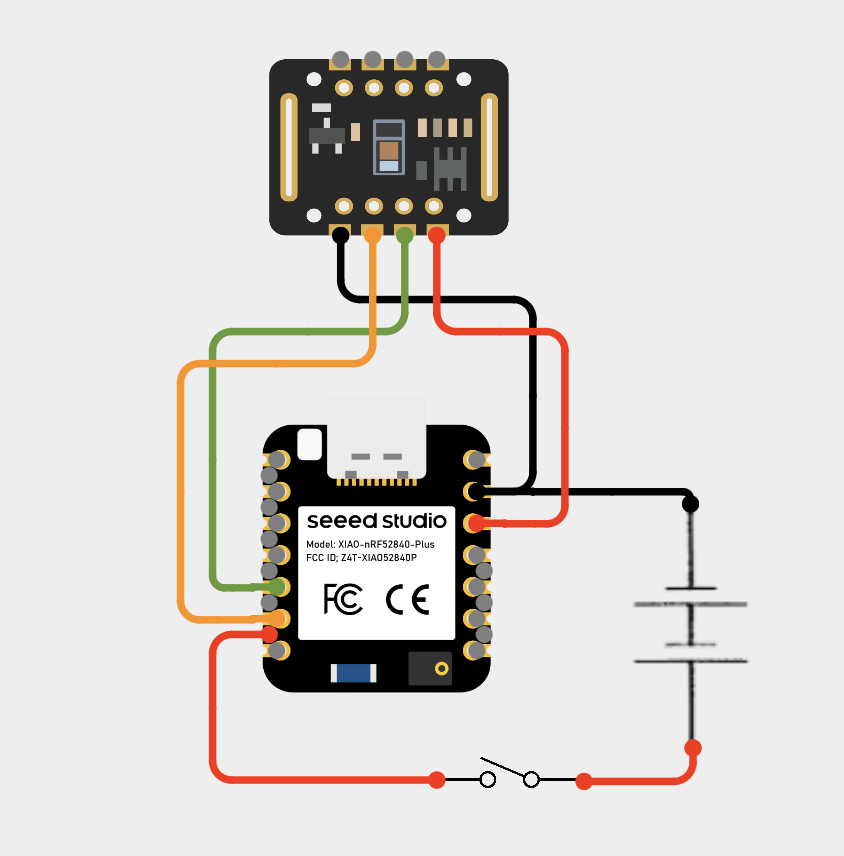
\includegraphics[width=0.5\textwidth]{img/fittag_circuit.png}
    \caption{Schema elettrico del FitTag Band.}
    \label{fig:schema_elettrico}
\end{figure}

\section{Architettura software}
Il firmware del dispositivo è sviluppato in linguaggio C++ sfruttando i vantaggi dell'ambiente integrato PlatformIO e del framework Arduino core per architetture nRF52. L'architettura software è stata progettata come una macchina a stati finiti e si appoggia a librerie specializzate per l'interfacciamento con i sensori e per la gestione del protocollo di comunicazione BLE.

\subsection{La Macchina a Stati Finiti}
La logica di controllo del sistema è orchestrata da una Macchina a Stati Finiti (FSM) che regola in modo deterministico le modalità operative del bracciale.
L'adozione di una FSM consente di implementare politiche attive di risparmio energetico: i sensori e i relativi canali di comunicazione vengono attivati, configurati o posti in modalità di sospensione hardware (sleep mode) esclusivamente quando strettamente richiesto dallo stato corrente.

La FSM è strutturata sui seguenti stati operativi:
\begin{itemize}
    \item \textbf{\texttt{INIT\_STATE}:} Stato transitorio iniziale. Una volta completato il setup, il sistema transita automaticamente verso lo stato di riposo \texttt{IDLE\_STATE}.
    \item \textbf{\texttt{IDLE\_STATE}:} Stato di standby a basso consumo energetico. In questa fase i sensori vengono spenti per preservare la carica della batteria. Questo stato è inoltre lo stato centrale dell FSM, in quanto qualsiasi transizione tra le diverse modalità operative della periferica deve necessariamente transitare attraverso questo stato.
    \item \textbf{\texttt{INFER\_STATE}:} Stato operativo in cui il sistema esegue on-device l'algoritmo di classificazione. L'IMU acquisisce i dati cinematici e li memorizza in un buffer temporaneo per consentire al modello di Machine Learning di stimare l'attività dell'utente in tempo reale.
    \item \textbf{\texttt{DATA\_LOG\_STATE}:} Stato finalizzato alla raccolta dati per l'addestramento offline del classificatore. Il microcontrollore campiona i segnali grezzi di accelerometro e giroscopio a $13\,Hz$ e li trasmette continuamente via BLE verso l'applicazione di raccolta.
    \item \textbf{\texttt{WORKOUT\_STATE}:} Stato attivo di monitoraggio dell'allenamento. In questa modalità vengono abilitati il contapassi hardware integrato nell'IMU e il sensore ottico per la rilevazione del battito cardiaco, calcolando e sincronizzando le metriche prestazionali a intervalli regolari.
    \item \textbf{\texttt{BATT\_LVL\_STATE}:} Stato transitorio deputato alla lettura della tensione della batteria tramite il convertitore analogico-digitale (ADC). La percentuale di carica residua calcolata viene inviata al client BLE prima di far ritornare automaticamente il dispositivo in \texttt{IDLE\_STATE}.
\end{itemize}

\begin{figure}[h!]
    \centering
    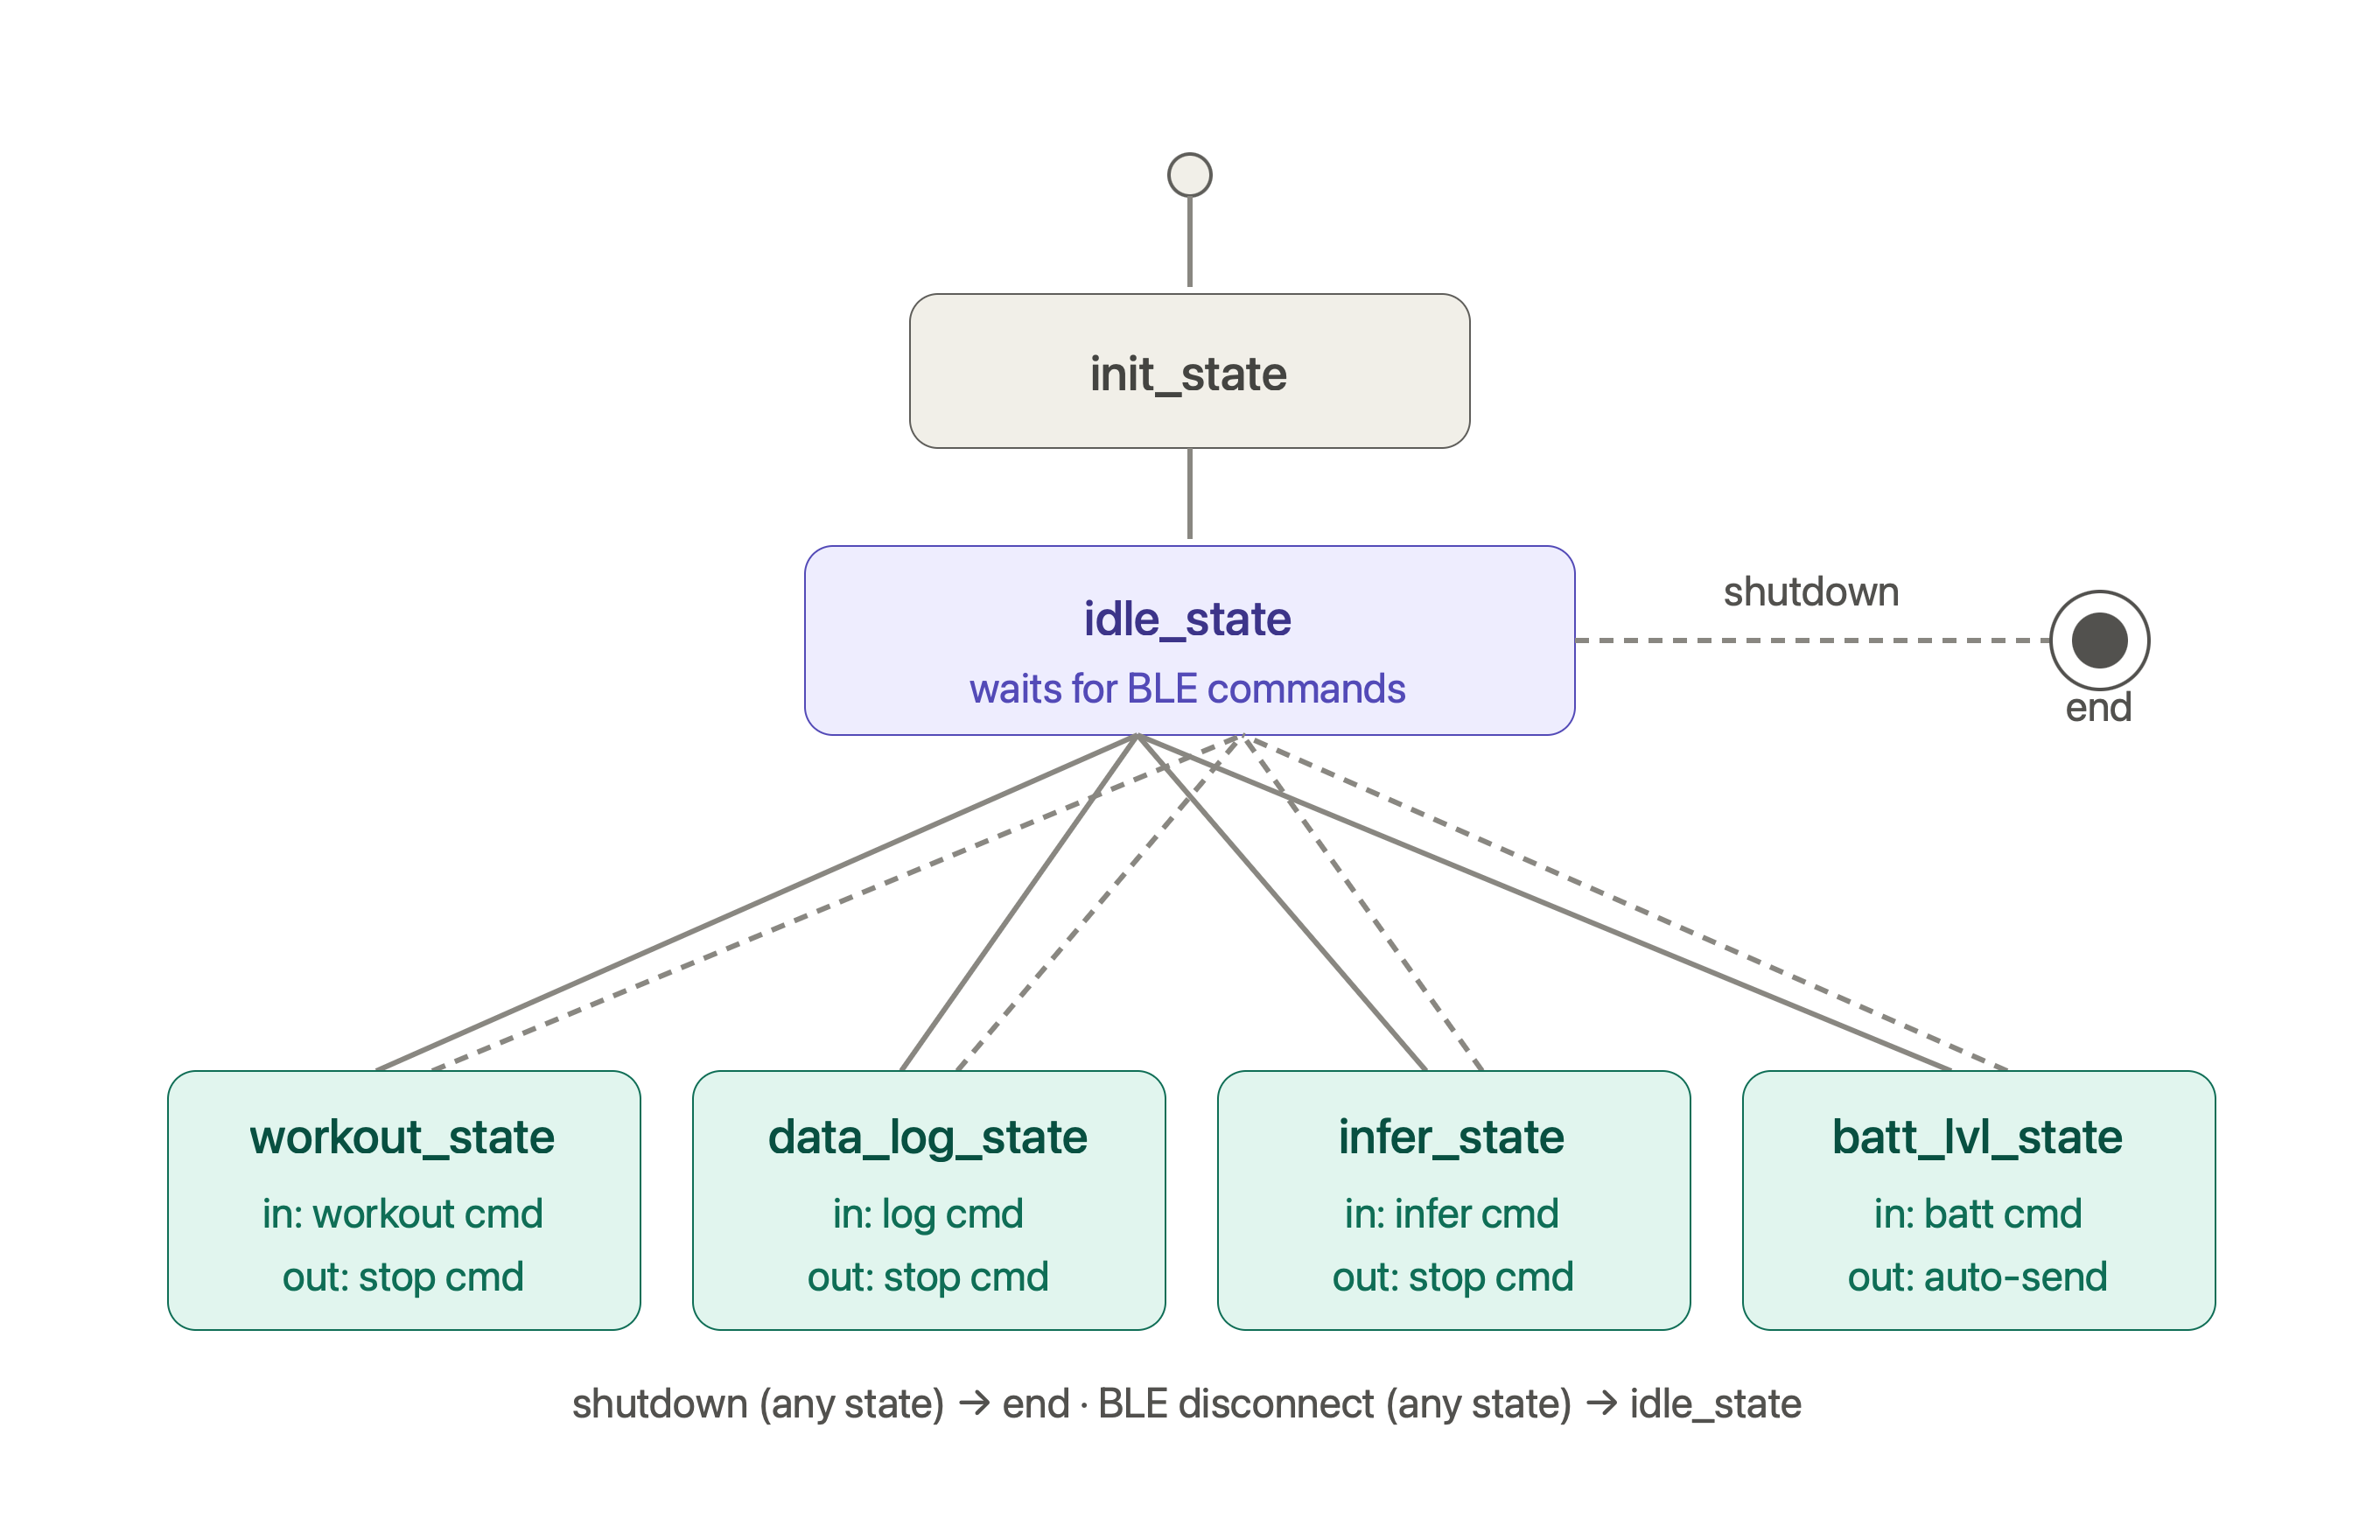
\includegraphics[width=0.55\textwidth]{img/fittag_fsm.png}
    \caption{Diagramma della Macchina a Stati Finiti del FitTag Band.}
    \label{fig:fittag_fsm}
\end{figure}

\subsection{Protocollo di comunicazione BLE}
L'interscambio dati tra il wearable e l'applicazione mobile è basato sul protocollo Bluetooth Low Energy (BLE). Il dispositivo FitTag Band è configurato per esporre un servizio primario custom (\texttt{fitTagService}).

Il servizio è strutturato in quattro caratteristiche distinte, ciascuna deputata a uno specifico flusso informativo:
\begin{itemize}
    \item \textbf{Control Characteristic (Write Only):} Permette all'applicazione mobile di inviare in modalità asincrona comandi di controllo di $1\,byte$. La ricezione di un comando attiva una routine di callback che valida la richiesta ed esegue la transizione di stato della macchina a stati finiti.
    \item \textbf{Inference Characteristic (Notify):} Utilizzata per trasmettere in tempo reale il risultato della classificazione effettuata dal modello integrato. Invia un pacchetto a lunghezza fissa di $1\,byte$ contenente l'ID dell'attività rilevata.
    \item \textbf{Data Log Characteristic (Notify):} Dedicata esclusivamente alla fase offline di raccolta dati cinematici. Sfrutta la modalità di notifica per inviare in modo efficiente array di strutture \texttt{IMUPayload} contenenti i campioni grezzi di accelerometro e giroscopio necessari per l'addestramento del modello.
    \item \textbf{Workout Characteristic (Notify):} Trasmette a frequenza di $1\,Hz$ la telemetria riepilogativa dell'allenamento (\texttt{WorkoutPayload}). Il pacchetto include il battito cardiaco filtrato, i passi totali registrati dal contapassi hardware, la cadenza calcolata e l'indice di intensità del movimento.
\end{itemize}

Oltre al servizio custom, il firmware inizializza il servizio standard di monitoraggio della batteria (\texttt{batteryService}), consentendo all'app mobile di accedere alle informazioni sul livello di carica.

\subsection{Scelte implementative e ottimizzazioni del firmware}

In questa sezione vengono analizzate le principali scelte architetturali e le ottimizzazioni di basso livello introdotte nel firmware del FitTag Band.

\subsubsection{Acquisizione dei dati sensoriali}
Al fine di massimizzare l'efficienza energetica del sistema e prolungare l'autonomia della batteria, l'architettura del firmware adotta un modello orientato agli eventi, eliminando la necessità di eseguire il polling continuo delle periferiche.

Nello specifico, la memoria interna del sensore viene configurata in modalità FIFO; al raggiungimento di una determinata soglia di riempimento, l'hardware dell'IMU genera un impulso elettrico sul pin fisico di interrupt.
Questo approccio consente al microcontrollore di permanere in uno stato di sospensione a basso consumo, riducendo drasticamente i cicli di clock sprecati in attesa della disponibilità del dato.
Il processore viene risvegliato dall'interrupt, esegue uno scaricamento a blocchi del buffer e rientra immediatamente nello stato di sleep.

Come mostrato nel frammento di codice~\ref{lst:imu_int}, tale comportamento viene configurato settando il bit \texttt{INT1\_FTH} del registro \texttt{INT1\_CTRL} dell'LSM6DS3TR-C, il quale instrada l'evento di raggiungimento della soglia FIFO direttamente sul pad hardware \texttt{INT1}.

\begin{lstlisting}[language=C++, caption={Configurazione del registro di controllo interrupt per l'unità inerziale.}, label=lst:imu_int]
// Abilitazione interrupt su soglia FIFO (bit INT1_FTH, valore 0x08) 
// e instradamento sul pin hardware INT1 dell'IMU
IMU.writeRegister(LSM6DS3_ACC_GYRO_INT1_CTRL, 0x08);
\end{lstlisting}

Al contrario, la gestione dei parametri vitali rilevati dal sensore MAX30102 segue una strategia differente. Poiché le metriche cardiache presentano dinamiche temporali significativamente più lente rispetto alle accelerazioni generate dal movimento corporeo, l'acquisizione dei dati viene demandata a un ciclo di polling a bassa frequenza, sufficiente a garantire la stabilità di calcolo dell'algoritmo di estrazione dei battiti al minuto senza gravare sul budget energetico complessivo del dispositivo.

\subsubsection{Configurazione del Block Data Update}
Un problema critico nei sistemi di acquisizione dati ad alta frequenza è la lettura di campioni corrotti dovuta al disallineamento temporale tra i registri a 8 bit di parte bassa (LSB) e parte alta (MSB) dei sensori.
Se la MCU esegue una lettura del registro LSB e, prima di completare la lettura del registro MSB, l'hardware del sensore aggiorna il dato a seguito di un nuovo ciclo di scrittura interno, il valore finale risulterà inevitabilmente falsato.

Per prevenire questo fenomeno, all'avvio della fase di logging il firmware configura esplicitamente il registro di controllo \texttt{CTRL3\_C} dell'LSM6DS3TR-C asserendo il bit \texttt{BDU} (Block Data Update):

\begin{lstlisting}[language=C++]
uint8_t ctrl3_c;
IMU.readRegister(&ctrl3_c, LSM6DS3_ACC_GYRO_CTRL3_C); 
ctrl3_c |= 0x40; // Asserzione del bit BDU
IMU.writeRegister(LSM6DS3_ACC_GYRO_CTRL3_C, ctrl3_c); 
\end{lstlisting}

Questa impostazione congela l'aggiornamento dei registri di output \texttt{OUT} finché la CPU non ha completato la lettura sequenziale di entrambe le metà dello stesso campione, garantendo la lettura atomica dei vettori cinematici.

\subsubsection{Calcolo dell'intensità dell'attività sportiva}
Durante lo stato operativo di allenamento (\texttt{WORKOUT\_STATE}), il sistema deve calcolare l'intensità istantanea dell'attività fisica dell'utente.
La lettura diretta dei singoli assi dell'accelerometro è tuttavia fortemente influenzata dall'orientamento spaziale del bracciale a causa dell'accelerazione di gravità sempre presente ($1\,g$). 

Per rendere la metrica di intensità indipendente dall'orientamento del dispositivo, il firmware implementa il calcolo della magnitudo del vettore risultante mediante la formula euclidea:
\begin{equation}
    totalG = \sqrt{a_X^2 + a_Y^2 + a_Z^2}
\end{equation}

Successivamente, viene applicata una logica di compensazione della gravità sottraendo il valore costante di $1.0\,g$:
\begin{equation}
    movement = |totalG - 1.0|
\end{equation}

Isolando unicamente la componente dinamica del movimento, il firmware mappa linearmente il punteggio su una scala discreta da 1 (completamente fermo) a 10 (massima intensità).

\subsubsection{Controllo del partitore di tensione per il sensing della batteria}
La lettura analogica della tensione della batteria nei dispositivi a basso consumo introduce una criticità progettuale legata al consumo parassita costante.
Un partitore di tensione resistivo tradizionalmente collegato in modo permanente provocherebbe infatti una scarica continua e lineare della batteria.
Tale fenomeno risulterebbe attivo anche quando l'unità centrale si trova in modalità sleep, compromettendo drasticamente l'autonomia complessiva del dispositivo.

Per ovviare a questo problema, l'architettura hardware del modulo Seeed Studio XIAO nRF52840 prevede la connessione di un ramo del partitore al pin digitale \texttt{VBAT\_ENABLE}.

Il firmware sfrutta questa topologia implementando una strategia di attivazione on-demand: il partitore viene chiuso verso massa unicamente per la finestra temporale strettamente necessaria al campionamento della tensione da parte del convertitore analogico-digitale.
Nella pratica, il pin \texttt{VBAT\_ENABLE} viene configurato come \texttt{OUTPUT} e settato a \texttt{LOW}. Questa transizione permette al pin di funzionare come pozzo di corrente, consentendo la corretta lettura della tensione.

Subito dopo l'acquisizione del dato, il pin viene forzato a livello logico \texttt{HIGH}. Il percorso di corrente verso la massa viene così interrotto, azzerando istantaneamente il consumo parassita.

\begin{lstlisting}[language=C++, caption={Implementazione software della lettura della tensione della batteria.}]
// Configurazione del pin di controllo e attivazione del partitore
pinMode(VBAT_ENABLE, OUTPUT);
digitalWrite(VBAT_ENABLE, LOW);

// Acquisizione del valore di tensione grezzo
int adc_value = analogRead(PIN_VBAT);

// Disattivazione del partitore
digitalWrite(VBAT_ENABLE, HIGH);
\end{lstlisting}

\subsubsection{Gestione della disconnessione BLE}
La perdita improvvisa della connessione wireless durante un allenamento o una fase di data logging comporta il rischio che il dispositivo rimanga bloccato in uno stato operativo. Questo scenario causerebbe un campionamento indefinito dei sensori e un rapido esaurimento della batteria.
Per prevenire questa condizione, il firmware implementa un meccanismo di fail-safe basato su una routine di callback asincrona (\texttt{disconnect\_callback}).

Al verificarsi della perdita di segnale radio con lo smartphone, la callback intercetta l'evento e forza la variabile asincrona \texttt{nextState} al valore \texttt{IDLE\_STATE}. Al ciclo successivo del \texttt{loop()}, il sistema rileva il cambio di stato ed esegue la routine \texttt{hardwareSleepMode()}.
Questo meccanismo garantisce che il wearable non rimanga mai bloccato in uno stato operativo in assenza di un host connesso.

\subsubsection{Gestione della sliding window per l'inferenza}
L'acquisizione dei dati per il modello Random Forest viene gestita tramite una finestra scorrevole (sliding window). La configurazione finale prevede una finestra temporale di $5\,s$ (pari a $65$ campioni acquisiti alla frequenza di $13\,Hz$) con una sovrapposizione di $2\,s$ ($26$ campioni).

Inizialmente, il modello era stato addestrato su finestre più corte, pari a $2\,s$ con $1\,s$ di overlap. Tuttavia, durante i test reali sul bracciale, si è verificato che estendere la finestra in fase di inferenza aumenta la precisione e la stabilità della classificazione.

I dati provenienti dai sensori vengono accumulati nella matrice \texttt{inferBuffer}. Quando il buffer raggiunge i $65$ campioni, il firmware estrae le features ed esegue l'inferenza. Per mantenere i $2\,\text{s}$ di overlap senza dover svuotare il buffer e attendere un riempimento completo, i dati più recenti vengono spostati all'inizio della matrice attraverso un ciclo di scorrimento:

\begin{lstlisting}[language=C++, caption={Scorrimento dei dati nel buffer per la gestione dell'overlap.}]
for (int k = 0; k < INFER_STEP_SIZE; k++) {
    for (int axis = 0; axis < 6; axis++) {
        inferBuffer[k][axis] = inferBuffer[k + INFER_STEP_SIZE][axis];
    }
}
inferBufferIndex = INFER_STEP_SIZE;
\end{lstlisting}

I dati più recenti (pari alla dimensione dello step) vengono copiati all'inizio del buffer, e l'indice di scrittura viene riposizionato a \texttt{INFER\_STEP\_SIZE}.
Questa tecnica garantisce un consumo di RAM costante e predefinito.

\subsubsection{Serializzazione dei dati e prevenzione del memory padding}
Per ottimizzare lo streaming wireless via BLE e rispettare i vincoli di dimensione imposti dalla Maximum Transmission Unit (MTU), è fondamentale minimizzare la dimensione dei pacchetti trasmessi. All'interno del file \texttt{sharedTypes.h}, le strutture dati \texttt{IMUPayload} e \texttt{WorkoutPayload} sono state dichiarate applicando la direttiva di compilazione \texttt{\_\_attribute\_\_((packed))}.

I compilatori per architetture a 32-bit, come il core ARM Cortex-M4 del SoC nRF52840, tendono ad allineare le variabili in memoria a indirizzi multipli di 4 byte, inserendo byte vuoti di riempimento (memory padding) per velocizzare i cicli di lettura della CPU. In un protocollo di rete, tuttavia, questo comportamento comporta due svantaggi critici: introduce un overhead inutile che consuma banda radio e altera la disposizione dei dati, impedendo una decodifica diretta da parte dell'applicazione mobile.

L'uso del modificatore \texttt{packed} forza il compilatore a rimuovere i byte di riempimento. In questo modo, la dimensione finale della struttura corrisponde alla somma esatta dei suoi tipi primitivi.

\section{Modello ML} % TODO: continuare da qui
La capacità di \textit{Human Activity Recognition} (HAR) del bracciale è resa possibile dall'implementazione \textit{on-device} di un classificatore ad albero, specificamente un \textit{Random Forest}, ottimizzato per l'esecuzione su sistemi embedded con risorse limitate (TinyML).

Il firmware applica un approccio a finestra temporale scorrevole (\textit{Sliding Window}) sui dati grezzi di accelerometro e giroscopio. Per campionamenti a 13 Hz, il sistema accumula dati in una finestra di 5 secondi (65 campioni). Per garantire una reattività ottimale mantenendo un contesto storico sufficiente, la finestra avanza con uno scivolamento (\textit{overlap}) di 2 secondi (26 campioni), permettendo di generare una nuova predizione regolarmente senza perdere ciclicità nel movimento.

Da ogni finestra temporale viene estratto un vettore di caratteristiche (\textit{features}) calcolando la media e la deviazione standard per ciascuno dei 6 assi inerziali. Il vettore risultante di 12 elementi in virgola mobile viene elaborato dal \textit{Random Forest}, il quale attraversa le diramazioni logiche generate in fase di addestramento e restituisce la classe di attività riconosciuta mediante un meccanismo di maggioranza sui voti degli alberi decisionali.